\documentclass[journal,10pt]{IEEEtran}
\usepackage{amsmath,amssymb,graphicx,booktabs,cite,url}
\newcommand{\RBR}{RBR}
\title{Rare-Reserved Balanced Replay for Federated Continual Intrusion Detection in EV Charging Networks}
\author{[Author names]\thanks{[Affiliations and contact information]}}
\markboth{Rare-Reserved Balanced Replay}{Federated Continual Intrusion Detection}
\begin{document}
\maketitle
\begin{abstract}
Small replay memories must preserve earlier intrusion patterns while retaining infrequent attacks. We evaluate rare-reserved balanced replay (RBR), which combines a fixed rare-group minimum with a class-balanced local remainder, for continual flow classification in electric-vehicle charging networks. At 60 examples per client, RBR improves old-attack accuracy by 1.53 percentage points and Slowloris recall by 5.06 points over class-balanced replay on the original split. Both federated gains remain significant on additional splits. Published class-balancing reservoir sampling and matched centralized controls extend the allocation comparison on one charging dataset with constructed client profiles.
\end{abstract}
\begin{IEEEkeywords}
Federated learning, continual learning, intrusion detection, replay memory, electric vehicle charging.
\end{IEEEkeywords}
\section{Introduction}
Charging stations depend on networked control and monitoring, making communication availability a security concern~\cite{ocpp,dataset}. Slowloris keeps incomplete HTTP requests open to consume server connection resources~\cite{slowloris}. Missing low-rate behavior can leave a service-disruption threat undetected even without a large traffic burst. A charging-network detector therefore needs to retain recognition of infrequent, previously encountered patterns as new attack classes arrive.

Federated training supports a shared detector while traffic remains at clients. D-IoT demonstrates federated IoT anomaly detection~\cite{diot}, and Kitsune studies online traffic anomaly detection~\cite{kitsune}. Continual intrusion detection also addresses forgetting and class imbalance through replay~\cite{amr}. We study how bounded client memories should allocate stored fitting flows under heterogeneous attack exposure.

Our contributions are: (i) a local rare-group reservation followed by a feasible class-balanced remainder; (ii) matched federated/centralized comparisons against uniform, class-balanced, protected and published CBRS population policies; and (iii) retention, Slowloris and worst-client results across memory capacities, attack orders and additional data-role splits.

\subsection{Related work}
FedAvg~\cite{fedavg}, FedProx~\cite{fedprox} and SCAFFOLD~\cite{scaffold} address distributed optimization; FedWeIT~\cite{fedweit} supports continual inter-client transfer. Small episodic memories~\cite{tiny} and exemplar-based incremental learning~\cite{icarl} motivate strong replay controls. GEM~\cite{gem}, A-GEM~\cite{agem}, EWC~\cite{ewc} and dark experience replay~\cite{der} modify gradients, regularization or stored targets.

CBRS balances a streaming reservoir and admits an importance-weighted extension~\cite{cbrs}; augmented replay studies imbalance-aware population and retrieval for IDS~\cite{amr}. RBR uses an explicit rare-group minimum followed by balanced task-boundary allocation. FedCBDR coordinates memory construction globally and changes logit scaling~\cite{fedcbdr}; RBR uses local candidates and the shared replay loss, with no allocation-related communication.

\section{Setting and Replay Allocation}
\subsection{Tasks and client profiles}
The MLP predicts benign and 14 attack types. Four cohorts are reconnaissance $R$ (aggressive, OS fingerprinting, SYN stealth, service-version and TCP-port scans), flooding $F$ (SYN, TCP, UDP, ICMP, PSHACK and synonymous-IP floods), low-rate/rare $L$ (Slowloris and ICMP fragmentation), and vulnerability scan $V$. Orders are $(R,F,L,V)$, $(F,R,V,L)$ and $(L,V,F,R)$. Benign fitting flows recur in each task. Unseen outputs are masked until their classes arrive.

Five constructed profiles emphasize reconnaissance, flooding or rare traffic, or are mixed or benign-starved. Table~\ref{tab:allocation} gives allocation weights; floors and largest-remainder redistribution assign each row to one client. All clients participate each round, and the global model is evaluated on each client's held-out flows.
\begin{table}[t]
\centering
\caption{Label-dependent client allocation weights (\%). Vulnerability uses the rare allocation row but is outside the reserved group.}
\label{tab:allocation}
\footnotesize
\begin{tabular}{lrrrrr}
\toprule
Group & Recon. & Flood & Rare & Mixed & Starved\\
\midrule
Benign &55&15&10&20&0\\
Reconnaissance &55&10&5&20&10\\
Flooding &10&55&5&20&10\\
Rare / vulnerability &5&5&55&25&10\\
\bottomrule
\end{tabular}
\end{table}

\subsection{Rare-reserved balanced replay}
At a task boundary, client $k$ forms candidates $C=\operatorname{unique}(M_{k,t-1}\cup D_{kt})$ from retained memory and current fitting rows. Let $B$ be capacity, $\mathcal G=\{\text{Slowloris},\text{ICMP fragmentation}\}$, and $\operatorname{Bal}(S,b)$ draw equal feasible quotas by cycling through original class labels, redistributing exhausted-class slots. RBR first reserves
\begin{align}
A&=\operatorname{Bal}(C^{\mathcal G},\min(\lfloor qB\rfloor,|C^{\mathcal G}|)),\\
M_{kt}&=A\cup\operatorname{Bal}(C\setminus A,B-|A|).
\end{align}
The balanced remainder includes benign and rare classes, so $q$ is a minimum reservation. Memory contains unique fitting flows and never exceeds $B$. Discarded history cannot re-enter except when it belongs to the current task's recurring benign reference.

With replay fraction $r$, local training minimizes $(1-r)\ell_{\rm current}+r\ell_{\rm replay}$ using cross-entropy and uniform sampling from retained rows. FedAvg weights updates by distinct current-plus-memory fitting counts. The centralized control pools all clients' fitting data and receives capacity $5B$, matching total replay storage.

\section{Experimental Protocol}
We cap each attack type at 3,000 available flows. The fixed sample has 36,172 rows: 23,513 fitting, 5,425 calibration and 7,234 evaluation. Persistent roles are stratified within client/type blocks using target fractions 0.65/0.15/0.20. Preprocessing excludes provenance, addresses, identifiers, absolute timestamps and fingerprint-like fields; scaling and categorical vocabularies fit only Task-1 fitting rows and then freeze. The backbone is input--64--32--15, ReLU and Adam, with five local epochs per round, five rounds per task, batch 128, weight decay $10^{-4}$ and no gradient clipping.

\subsection{Comparators and calibration}
The replay comparison varies memory allocation under a fixed replay loss. EWC, A-GEM and DER++ modify regularization, gradients or replay targets; their mechanisms are complementary and could be combined with the allocation rule. We report EWC and A-GEM as additional learning references. Joint fitting uses all tasks' fitting rows from the start.

Uniform replay samples candidates randomly; class-balanced applies $\operatorname{Bal}$ to the whole pool. Protected reserves 20\% each for benign and the rare group, then fills randomly. RBR calibrates $q\in\{0.10,0.20\}$; replay methods calibrate $r\in\{0.25,0.50\}$ at learning rate 0.003. Choices maximize mean-checkpoint original-type calibration macro recall, separately for each environment/order/capacity. Fine-tuning and joint calibrate learning rate in $\{0.001,0.003\}$; EWC calibrates $\lambda\in\{1,100\}$ and A-GEM reference batch size in $\{32,64\}$.

CBRS uses the published population rule~\cite{cbrs}: once memory is filled, non-full classes replace a random member of a largest class, while full classes use within-class reservoir replacement with probability $m_c/n_c$. A class remains full after becoming largest in filled memory. Each fitting flow enters the population stream once, counters persist, and population updates occur at the shared task boundary. CBRS calibrates only $r$ on original split 42, at $B=60$, under the same backbone and replay loss. All settings are selected before evaluation.

\subsection{Scoring}
Primary scoring sums six scan probabilities into one Scan output: the five reconnaissance types and vulnerability scan. Slowloris remains separate; original type labels and task cohorts are retained for training. A scan-only Random Forest achieves 34.25\% evaluation accuracy while fitting perfectly, motivating merged reporting alongside exact-type sensitivity.

Old accuracy averages final attack accuracy over the first three original cohorts. Forgetting averages each cohort's maximum post-learning accuracy minus its final accuracy. Slowloris recall uses its 600 evaluation flows. Worst-client score is the minimum supported-class macro recall. We report means and sample SD over ten training-seed averages of three orders; paired 95\% $t_9$ intervals use the ten seed differences. Additional role-split seeds 43--45 preserve the sample, allocation and settings, refit Task-1 preprocessing, and recalibrate the key RBR/class-balanced comparison at $B=60$.

\section{Results}
\begin{table}[t]
\centering
\caption{Federated memory 60/client, original split 42. Merged-Scan scores (\%); mean $\pm$ SD of ten seed averages over three orders. Worst is client macro recall.}
\label{tab:main}
\footnotesize
\setlength{\tabcolsep}{2.5pt}
\begin{tabular}{lrrrr}
\toprule
Method & Old acc. $\uparrow$ & Forget $\downarrow$ & Slowloris $\uparrow$ & Worst $\uparrow$\\
\midrule
No replay & 22.22 $\pm$ 0.00 & 77.60 $\pm$ 0.02 & 33.33 $\pm$ 0.00 & 14.81 $\pm$ 0.00\\
Uniform & 65.29 $\pm$ 2.92 & 34.53 $\pm$ 2.93 & 66.98 $\pm$ 7.02 & 45.50 $\pm$ 2.86\\
Class-balanced & 83.99 $\pm$ 1.44 & 15.77 $\pm$ 1.42 & 71.56 $\pm$ 4.19 & 77.97 $\pm$ 1.05\\
CBRS & 83.88 $\pm$ 1.12 & 15.89 $\pm$ 1.12 & 72.57 $\pm$ 2.04 & 77.87 $\pm$ 1.50\\
Protected & 72.84 $\pm$ 2.25 & 26.84 $\pm$ 2.29 & 82.73 $\pm$ 2.36 & 47.15 $\pm$ 3.82\\
RBR & 85.52 $\pm$ 1.27 & 14.24 $\pm$ 1.27 & 76.62 $\pm$ 4.16 & 79.03 $\pm$ 1.00\\
EWC & 24.89 $\pm$ 1.30 & 74.95 $\pm$ 1.30 & 33.33 $\pm$ 0.00 & 17.15 $\pm$ 3.56\\
A-GEM & 46.03 $\pm$ 4.58 & 53.80 $\pm$ 4.58 & 50.29 $\pm$ 4.68 & 37.12 $\pm$ 3.29\\
Joint & 94.20 $\pm$ 0.07 & -- & 76.82 $\pm$ 0.17 & 77.89 $\pm$ 1.48\\
\bottomrule
\end{tabular}
\end{table}

\begin{table}[t]
\centering
\caption{Federated memory 60, original split. Both views (\%, mean $\pm$ SD); CB denotes class-balanced.}
\label{tab:type}
\footnotesize
\setlength{\tabcolsep}{1.5pt}
\begin{tabular}{llrrrr}
\toprule
Method & View & Old acc. & Forget & Slowloris & Worst\\
\midrule
CB & Merged & 83.99 $\pm$ 1.44 & 15.77 $\pm$ 1.42 & 71.56 $\pm$ 4.19 & 77.97 $\pm$ 1.05\\
CBRS & Merged & 83.88 $\pm$ 1.12 & 15.89 $\pm$ 1.12 & 72.57 $\pm$ 2.04 & 77.87 $\pm$ 1.50\\
RBR & Merged & 85.52 $\pm$ 1.27 & 14.24 $\pm$ 1.27 & 76.62 $\pm$ 4.16 & 79.03 $\pm$ 1.00\\
CB & Exact & 47.68 $\pm$ 1.68 & 34.97 $\pm$ 1.67 & 72.25 $\pm$ 4.12 & 51.71 $\pm$ 0.72\\
CBRS & Exact & 49.35 $\pm$ 1.14 & 32.31 $\pm$ 1.02 & 74.70 $\pm$ 3.87 & 51.47 $\pm$ 0.89\\
RBR & Exact & 49.58 $\pm$ 1.97 & 33.08 $\pm$ 1.99 & 78.27 $\pm$ 5.01 & 52.41 $\pm$ 0.69\\
\bottomrule
\end{tabular}
\end{table}

\subsection{Retention and Slowloris at memory 60}
RBR reaches 85.52\% old accuracy and 76.62\% Slowloris recall. Over class-balanced, gains are $+1.53$ points $[0.23,2.84]$ for old accuracy and $+5.06$ $[1.27,8.84]$ for Slowloris; forgetting falls by 1.54 points. Worst-client difference is $+1.06$ $[-0.07,2.19]$. Exact-type scores appear in Table~\ref{tab:type}.

Against protected, RBR gains 12.68 points of old accuracy and 31.87 of worst-client score, while losing 6.11 points of Slowloris. The rare+random/no-benign ablation reaches 72.07\% old accuracy, 84.78\% Slowloris and 48.62\% worst-client score: RBR changes these by $+13.45$, $-8.16$ and $+30.41$ points, respectively, with all three paired intervals excluding zero. This exposes the retention--Slowloris trade-off of random filling.

Federated RBR minus CBRS differences are old accuracy $+1.64$ $[0.40,2.88]$, Slowloris $+4.04$ $[0.41,7.68]$, and worst-client $+1.16$ $[0.02,2.30]$. Centralized RBR minus CBRS differences are old accuracy $+3.25$ $[2.21,4.30]$, Slowloris $+7.93$ $[4.09,11.77]$, and worst-client $+0.49$ $[-0.68,1.66]$. In centralized order 2, the slowloris recall difference is $-0.58$ $[-1.07,-0.10]$. With exact types, federated old-accuracy and Slowloris differences are $+0.23$ $[-1.75,2.21]$ and $+3.57$ $[-0.92,8.06]$; both intervals include zero.

\subsection{Capacity, order and federation}
\begin{table}[t]
\centering
\caption{Memory 300/client, same setting and scoring as Table~\ref{tab:main}.}
\label{tab:capacity}
\footnotesize
\setlength{\tabcolsep}{2.5pt}
\begin{tabular}{lrrrr}
\toprule
Method & Old acc. $\uparrow$ & Forget $\downarrow$ & Slowloris $\uparrow$ & Worst $\uparrow$\\
\midrule
Class-balanced & 88.26 $\pm$ 0.76 & 11.43 $\pm$ 0.77 & 83.43 $\pm$ 1.02 & 81.48 $\pm$ 1.29\\
Protected & 91.24 $\pm$ 0.52 & 8.15 $\pm$ 0.64 & 94.45 $\pm$ 1.97 & 75.72 $\pm$ 1.43\\
RBR & 89.94 $\pm$ 0.98 & 9.50 $\pm$ 1.08 & 89.37 $\pm$ 2.87 & 81.91 $\pm$ 1.34\\
\bottomrule
\end{tabular}
\end{table}

At memory 300, RBR improves old accuracy, Slowloris and worst-client score over class-balanced by 1.68, 5.94 and 0.42 points, respectively; each interval excludes zero. Protected exceeds RBR on old accuracy and Slowloris by 1.30 and 5.08 points, while RBR retains a 6.19-point worst-client advantage.
\begin{figure}[t]
\centering
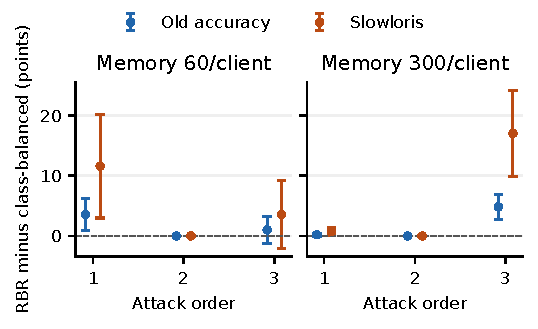
\includegraphics[width=\columnwidth]{figures/order_effects.pdf}
\caption{RBR minus class-balanced by order and capacity, original split. Bars are paired 95\% intervals over ten seeds.}
\label{fig:orders}
\end{figure}
Fig.~\ref{fig:orders} shows order variation. At memory 60, Slowloris gains are 11.60, 0 and 3.57 points across the three orders; order 2 ends with the rare cohort, where both methods reach full recall. At memory 300, RBR loses old accuracy to protected in orders 1 and 2.

The gains hold under federated heterogeneity and align with centralized controls at matched total storage. Centralized RBR gains over class-balanced at memory 60 are 1.67 points of old accuracy and 5.00 of Slowloris. Federated-minus-centralized differences in improvement are $-0.14$ $[-1.54,1.26]$ and $+0.06$ $[-4.26,4.38]$, respectively. Table~\ref{tab:splits} shows positive retention and Slowloris differences on all four splits in both settings; both federated gains are significant on each split. Centralized significance varies across splits. The rare-heavy/benign-starved profiles have RBR macro recall 79.25/88.55\%, versus 78.30/88.58\% with class-balanced replay.
\begin{table}[t]
\centering
\caption{RBR minus class-balanced at memory 60; percentage points [95\% paired interval].}
\label{tab:splits}
\footnotesize
\setlength{\tabcolsep}{3pt}
\begin{tabular}{llrr}
\toprule
Split & Setting & Old accuracy & Slowloris\\
\midrule
42 & Fed. & $+1.53$ $[0.23,2.84]$ & $+5.06$ $[1.27,8.84]$\\
42 & Central & $+1.67$ $[1.12,2.22]$ & $+5.00$ $[3.04,6.96]$\\
43 & Fed. & $+2.23$ $[0.95,3.51]$ & $+7.93$ $[4.03,11.83]$\\
43 & Central & $+1.11$ $[0.47,1.74]$ & $+3.48$ $[1.31,5.65]$\\
44 & Fed. & $+3.37$ $[2.11,4.63]$ & $+11.28$ $[7.59,14.97]$\\
44 & Central & $+1.13$ $[-0.19,2.46]$ & $+3.80$ $[-0.79,8.39]$\\
45 & Fed. & $+2.06$ $[0.40,3.72]$ & $+6.09$ $[1.30,10.88]$\\
45 & Central & $+0.82$ $[0.01,1.63]$ & $+2.61$ $[-0.01,5.22]$\\
\bottomrule
\end{tabular}
\end{table}


\section{Limitations and Conclusion}
The overlapping random splits use one dataset and constructed clients, not independent captures. Source filenames provide file groups, but no explicit session/capture column was found; only two benign and two Slowloris files prevent all three roles from having whole-file support. Sixteen benign and five fragmentation evaluation flows preclude false-alarm and fragmentation claims. Task-1 categorical vocabularies differ by order, mixing representation and order effects. Client results are descriptive; non-significance does not establish non-inferiority, and intervals are unadjusted for multiple comparisons.

CBRS population is assessed under the shared task-boundary training protocol and uniform replay retrieval; the original paper's separate weighted-replay training recipe is outside this comparison. Its federated retention/Slowloris significance depends on merged scoring. The rare+random ablation also varies calibrated quotas and within-group sampling, limiting single-component causal attribution. EWC was calibrated over a limited lambda range. FedCBDR's public image/CUDA checkout requires reconstruction for a faithful tabular baseline. Replay capacity counts rows, not total RAM; deployment, attack blocking and privacy guarantees are not measured.

RBR improves retention and Slowloris over class-balanced across the tested federated splits. Published CBRS and allocation ablations sharpen the comparison, while all losses remain part of the evidence. The result is a local replay-allocation policy evaluated under heterogeneous charging-network flow distributions.

\noindent\textbf{Code and data availability.} Code, configurations and split manifests: \url{https://github.com/f20230006-sketch/evse-fcl-multiclass-pilot} (private repository; access required). Dataset source:~\cite{dataset}.

\IEEEtriggeratref{12}
\begin{thebibliography}{18}
\bibitem{ocpp} Z. Garofalaki, D. Kosmanos, S. Moschoyiannis, D. Kallergis, and C. Douligeris, ``Electric vehicle charging: A survey on the security issues and challenges of the Open Charge Point Protocol (OCPP),'' arXiv:2207.01950, 2022, doi: 10.1109/COMST.2022.3184448.
\bibitem{dataset} Canadian Institute for Cybersecurity, ``CIC EV charger attack dataset 2024 (CICEVSE2024),'' University of New Brunswick, 2024. [Online]. Available: \url{https://www.unb.ca/cic/datasets/evse-dataset-2024.html}
\bibitem{slowloris} R. Giobbi, ``Mitigating Slowloris,'' 2009. [Online]. Available: \url{https://www.sei.cmu.edu/blog/mitigating-slowloris/}
\bibitem{diot} T. D. Nguyen \emph{et al.}, ``D-IoT: A federated self-learning anomaly detection system for IoT,'' in \emph{Proc. IEEE ICDCS}, pp. 756--767, 2019, doi: 10.1109/ICDCS.2019.00080.
\bibitem{kitsune} Y. Mirsky, T. Doitshman, Y. Elovici, and A. Shabtai, ``Kitsune: An ensemble of autoencoders for online network intrusion detection,'' in \emph{Proc. NDSS}, 2018, doi: 10.14722/ndss.2018.23204.
\bibitem{amr} S. K. Amalapuram, S. S. Channappayya, and B. R. Tamma, ``Augmented memory replay-based continual learning approaches for network intrusion detection,'' in \emph{Advances in Neural Information Processing Systems}, vol. 36, 2023.
\bibitem{fedavg} B. McMahan, E. Moore, D. Ramage, S. Hampson, and B. A. y Arcas, ``Communication-efficient learning of deep networks from decentralized data,'' in \emph{Proc. AISTATS}, PMLR, vol. 54, pp. 1273--1282, 2017.
\bibitem{fedprox} T. Li \emph{et al.}, ``Federated optimization in heterogeneous networks,'' in \emph{Proc. MLSys}, vol. 2, 2020.
\bibitem{scaffold} S. P. Karimireddy \emph{et al.}, ``SCAFFOLD: Stochastic controlled averaging for federated learning,'' in \emph{Proc. ICML}, PMLR, vol. 119, pp. 5132--5143, 2020.
\bibitem{fedweit} J. Yoon, W. Jeong, G. Lee, E. Yang, and S. J. Hwang, ``Federated continual learning with weighted inter-client transfer,'' in \emph{Proc. ICML}, 2021, arXiv:2003.03196.
\bibitem{tiny} A. Chaudhry \emph{et al.}, ``On tiny episodic memories in continual learning,'' arXiv:1902.10486, 2019.
\bibitem{icarl} S.-A. Rebuffi, A. Kolesnikov, G. Sperl, and C. H. Lampert, ``iCaRL: Incremental classifier and representation learning,'' in \emph{Proc. CVPR}, pp. 2001--2010, 2017.
\bibitem{gem} D. Lopez-Paz and M. Ranzato, ``Gradient episodic memory for continual learning,'' in \emph{Advances in Neural Information Processing Systems}, vol. 30, 2017.
\bibitem{agem} A. Chaudhry, M. Ranzato, M. Rohrbach, and M. Elhoseiny, ``Efficient lifelong learning with A-GEM,'' in \emph{Proc. ICLR}, 2019.

\bibitem{ewc} J. Kirkpatrick \emph{et al.}, ``Overcoming catastrophic forgetting in neural networks,'' \emph{Proc. Natl. Acad. Sci. USA}, vol. 114, no. 13, pp. 3521--3526, 2017, doi: 10.1073/pnas.1611835114.
\bibitem{der} P. Buzzega, M. Boschini, A. Porrello, D. Abati, and S. Calderara, ``Dark experience for general continual learning: A strong, simple baseline,'' in \emph{Advances in Neural Information Processing Systems}, vol. 33, 2020.
\bibitem{cbrs} A. Chrysakis and M.-F. Moens, ``Online continual learning from imbalanced data,'' in \emph{Proc. ICML}, PMLR, vol. 119, pp. 1952--1961, 2020.
\bibitem{fedcbdr} Z. Qi, Y.-P. Tang, L. Meng, H. Yu, X. Li, and X. Meng, ``Class-wise balancing data replay for federated class-incremental learning,'' arXiv:2507.07712, 2025.
\end{thebibliography}

\end{document}
